\chapter{Méthodes}
\label{chap:resultats_comparaisons}


\section{Proteus}


Proteus est constitué de deux parties:

\begin{enumerate}
\item un ensemble de scripts XPLOR, qui controle le calcul de la matrice d'énergie. (XPLOR est un programme de simulation moléuclaire (\ref{}), disponible en téléchargement sur le site de l'université de Yale).
\item un programme écrit en C ,que nous appelons \og proteus\fg dans la suite de ce texte, qui explore l'espace de sequence/conformation
\end{enumerate}

Le logiciel est flexible et largement configurable; Il permet l'utilisation de plusieurs champ de force, de plusieurs modèle de solvant, et de plusieurs librairie de rotamer.La partie en C, proteus, propose plusieurs algorithme d'exploration comme l'heuristique, MC ou REMC .Le programme proteus permet de diviser le système en plusieurs groupes ou d'en dupliqué une partie , ceux-ci pouvant alors être combiné dans la fonction d'énergie afin de favoriser la stabilité de certains sous-ensembles du système ou certaines affinités.
Plusieurs succès ont déjà était obtenue avec Proteus par exemple de redesign de la tyrosyl-tARN synthetase (\ref{}) ou sur la D-tyrosine ref{}, sur les cacluls de pK_a \ref{31}.

Nous detaillons les points importants de Proteus.

Notre logiciel Proteus autorise le choix entre plusieurs type de fonction d'énergie.Dans le type le plus simple \ogMMCASA\fg, est combinée l'approche de la mécanique moléculaire pour le traitement de la protéine et un modèle de solvant implicite de type CASA (voir  ~\ref{}). Deux types \ogLLGBSA\fg sont égalament possible , dans lesquels le traitement du solvant est effectuée par un modèle Born Genéralisé, avec soit une approximation NEA pour les rayons de sovatation, soit une approximation FDB.
Comme il a était vu précédement, avoir une fonction d'énergie décomposable par paire a plusieurs avantages, en particulier le calcul des énergies des paires de résidues avant l'étape d'exploration permet de reduire le calcul de l'énergie d'une séquence conformation pendant celle-ci à une somme d'énergies pré-calculées. Cependant les termes GB et SA ne sont pas décomposable par paire. Il faut alors introduite de nouvelles approximation pour le permettre.Nous allons dans la suite comment ces problèmes sont résolues dans Proteus.
\subsection{décomposotion en paire du terme de surface}
Le terme surfacique présenté en (~\ref{0}) ce défini comme:

\begin{equation}
E_{solv}^\surf = \sum_i \sigma_{t_i} A_i 
\end{equation}
avec $A_i$ la surface accessible au solvant de l'atome $i$, et $\sigma_{t_i}$ un coefficient d'hydrophobicité du type de l'atome $i$.
Ce terme n'est pas décomposable par paire de résidu, parce que  la surface enfouie d'une première chaîne latérale par une chdeuxième  peut aussi être enfuie par troisième chaîne latérale. Pour rendre ce terme décomposable, nous utilisons la méthode de Street et al (~\ref[41]), dans laquelle la surface enfuie d'une chaîne est calculée à partir d'une somme sur les chaîne et les groupes du backbone voisins.Puis pour chaque groupe voisins, la zone de contact avec notre chaîne est calculée indépendament des autres groupes. Ces zones sont sommées et un facteur de contraction est appliqué mimant l'élimination des zones comptée à plusieurs reprise.Des travaux précédents effectuée dans notre laboratoire ont montré qu'un facteur de 0,65 fonctionne bien (37, 40).   

\subsection{\og Native Environnement Approximation\fg (NEA)}

Dans le terme GB de l'énergie de solvatation, le rayon de solvatation $b_i$ approche la distance de l'atome $i$ à la surface de la protéine, et donc c'est une fonction de la position relative à $i$ de tous les atomes de la protéine.Et ce rayon n'est pas décomposable par paire.Pour qu'il ne devienne, Proteus utilise l'approximation  \og Native Environnement Approximation\fg ou NEA, dans laquelle le rayon de solvatation de chaque chaîne latérale est calculé avant l'étape d'exploration, en fixant tout le reste du système dans sa séquence native et sa conformation native[27,40]. 


\subsection{\og Fluctuating Dielectric Boundary\fg (FDB)}

Une nouvelle approximation du GB a récement été introduite dans Proteus, toujours avec l'objectif, de transformer ce terme en en terme additif par paire.Elle exploite le fait que dans le GB, l'environement dielectrique  d'une paire de résidue est completement caractérisé pour un petit ensemble de rayon de solvatation d'atome.Ces rayons sont eux-mêmes sommes de paire sur les atomes de la protéines voir 14 16.La méthode s'appelle Fluctuating Dielectric Boundary\fg ou FDB  et comporte les deux étapes suivantes:

La premiere consiste à définir un rayon de solvatation $B_I$ pour chauqe résidu $I$ de la protéine.

On commence par définir une énergie propre à chaque paire de résidus I,J par la somme suivante:

  \begin{equation}
    E_\IJ^{self} = \sum_{i\in I,j\in J} E_\ij^\self
  \end{equation}
  puis l'énergie propre d'un résidu I:

  \begin{equation}
    E_\I^{self} = \sum_J E_\ij^\self
  \end{equation}
    
  Alors le rayon de solvatation moyen $B_I$ est défini par:
\begin{equation}
    E^{self}_I \stackrel{def}{=} \tau \sum_{i \in I} \frac{q_i^2}{2 B_I}.
\end{equation} 

Nous avons, alors

\begin{equation}
\left( \sum_{i \in I} q_i^2 \right) \frac{1}{B_I} = \sum_{i \in I} \frac{q_i^2}{b_i}.
\end{equation}

Donc, $B_I$ est la moyenne harmonique des $b_i$, avec $i \in I$, pondéré par les charges au carré.

Il et alors possible de définir la contribution $g_\IJ$ de la paire de résidu I et J à l'énergie d'écrantage total $\Delta^\solv$, par:

\begin{equation} 
g_{IJ} = \sum_{i \in I, j \in J} \tau q_i q_j \left( r_{ij}^2 + B_I B_J \exp[-r_{ij}^2/4 B_I B_J] \right)^{-1/2}
\label{eq:screen}
\end{equation}

Avec, la somme pour $I=J$ excluant le cas $i \neq j$.
On peut noter qu' aux distances fixes $r_\ij$, et avec $B=B_IBJ$, $ g_\IJ (B)$ varie faiblemement en fonction de B. Simonson et al (dans 54), propose alors d'approximer cette fonction par:

\begin{equation}
  \label{eq:approx}
g_{IJ}(B) \approx c_1^{IJ} + c_2^{IJ} B + c_3^{IJ} B^2 + c_4^{IJ} B^{-1/2} + c_5^{IJ} B^{-3/2}  \label{eq:approx}
\end{equation}

Les coefficients $c_n^{IJ}$ peuvent alors être pré-calculé est stocké dans la matrice d'énergie, puisque les distances $r_\ij$ ne sont pas des variables pour un couple de chaîne latérale I,J donné. 
Comme les rayons de solvatation d'un résidu sont eux-mêmes des sommes sur les paires, le calcul de l'énergie GB à l'aide de \ref{eq:approx} est maintenant décomposable par paire.


\subsection{La matrice d'énergie}

Proteus utlise d'une part un backbone fixe, une espace discrét de rotamère et une fonction d'énergie décomposable par paires. Ces trois élèment permetent de pré-calculer toutes les énergies interactions possibles. A cet ensemble d'interactions , il faut ajouter les interactions des résidues avec le backbone ceci pour chacun des rotamères possibles, pour constituer un ensemble complet de valeur énergétiques qui permet d'obtenir la valeur de la fonction d''énergie pour chaque sequence/conformation.Cet ensemble peut être organisée sans le format d'une matrice symétrique dans laquelle chaque couple de position dans la chaîne polypeptidique, apparait avec sa multiplicité de couples de rotamères possibles voir ~\ref{Graph:mat_ener}.      

Le calcul de la matrice d'énergie, sont executer à l'aide du programme X-plor; il se déroule de la façon suivante:


   \begin{figure}[t]
     \centering
     \begin{tabular}{cc}
       
\includegraphics[width=12cm]{graphe/proteus/matrice.png} &
     \end{tabular}
     
     \caption{\textbf{La matrice d'énergies}Sur cet exemple, un polypeptide de 6 résidues, chaque position posséde type d'acide aminés possibles et 3 rotamères possibles (2 pour le type A et 1 pour le type B). La matrice organise toutes les interactions de paires de chaîen latérales possibles. Les interactions impliquant le résidu numéro 2 sont dans la bande jaune de la matrice, les interactions impliquant le résidu numéro 3 sont dans la bande bleue.Les points rouge et vert correspondent aux interactions  noté par les flèches rouge et verte à gauche(La matrice est symétrique , ici les interactions sont reprrésentées qu'une seule fois).}
\label{graph:MAt_ener}
   \end{figure}
   

- Les atomes du squelette , c'est à dire les N,H,$C_\alpha$ ,C et O , sont fixés une fois pour toute. 
- Les atomes des chaînes latérales sont placés avec les angles dièdres issue de la bibliothèque de rotamères de Tuféry (~\ref{20}).
- La fonction d'énergie qui utilise le champ de force Amber \ref{..} de la forme:

\begin{equation} \label{eq:energy}
E = E_{bonds} + E_{angles} + E_{dihe} + E_{impr} + E_{vdw} + E_{Coul} + E_{solv} 
\end{equation}

avec $E_{solv}$ pouvant être obtenu par le modèle CASA , le modèle GBNEASA ou GBFDBSA , correspondant respectivement à la formule \ref{eq:CASA},\ref{eq:NEA} et \ref{eq:FDB}, ceci selon la configuration de l'utilisateur.


\subsection{l'état déplié}

le $\Delta \Delta G$ du chapitre précédent, s'applique entre l'état replié de la protéine et un état déplié. Nous avons donc besoin d'attribuer une énergie à l'état déplié.Cet état ne correspond pas à une structure précise pour une certaine séquence d'acide aminé. de même on peut considérer que pour un résidu donné la position les deux résidues immédiatement de doit pas impacter fortement l'énergie.Cela inspire une definition indépendante la structure telle que:
\begin{equation}
E_u(S) = \sum_i^N E(t_i)  
\end{equation}

avec $E(t_i)$ une énergie du type d'acide aminé $t_i$.

Ces énergies est prise en entrée dans Proteus, et donc sa détermination ne fait pas encore partir des fonctionnalité intégré à notre logiciel.Il apparaît clairement dans la suite que la determination doit être fonction du système étudier. Nous detaillerons dans le chapitre PDZ, plusieurs méthodes dont de nouvelles et plusieurs exemple de determination qui seront exploitées.



\subsection{déroulemement de la construction de la matrice}

A partir un fichier PDB, une série de script XPLOR va préparer le système, ce système peut contenir un ligand.

\begin{enumerate}
-1- L'utilisateur configure l'execution:
Il determine:
\begin{itemize}
\item un champ de force. Les champs AMBER ff99SB ou CHARMM toph19 sont tous les deux supportés.
\item un modèle de solvant parmi CA GBNEA GBFDB
\item un jeu de coefficients \sigma_i pour la pondération de la surface accessible au solvant dans le terme hydrophobe.
\item l'ensemble des résidus dans le backbone autorisé à muter
\item l'ensemble des chaînes laterales autorisé à se déplacer 
\end{itemize}


-2- Pour chaque résidu, un ensemble de conformation est défini à partir d'une librairie de rotamer. Cet ensemble est sauvegardé dans un fichier PDB par position.

-3- Les rayons de solvatation de Born sont calculé selon l'approximation GB demandé. Ces rayons sont sauvegardé dans un fichier dédié.
-4- pour chaque rotamére de chaque type, après une petite minimisation, est calculée ou lui seul peut se déplacer, l'énergie d'interaction avec le squelette.Elle est stocké dans une fichier.Ce sont les énergies de la diagonale de matrice.l'objectif de la minimisation est d'adapter le rotamère à son environement natif.
-5- Pour chaque paire de rotamère possible,comme pour la diagonale de ma matrice, une petite minimisation est effectuée avec uniquement la paire courante qui peut se deplacer.Puis les termes d'énergie d'interaction du couple sont  calculés et enregistrés dans du fichiers.  
\end{enumerate}
  
Ensuite , les differents fichiers d'énergies seront lu par proteus voir \ref{} pour construire la matrice.

\subsection{les groupes dans proteus}
   \begin{figure}[t]
     \centering
     \begin{tabular}{cc}
       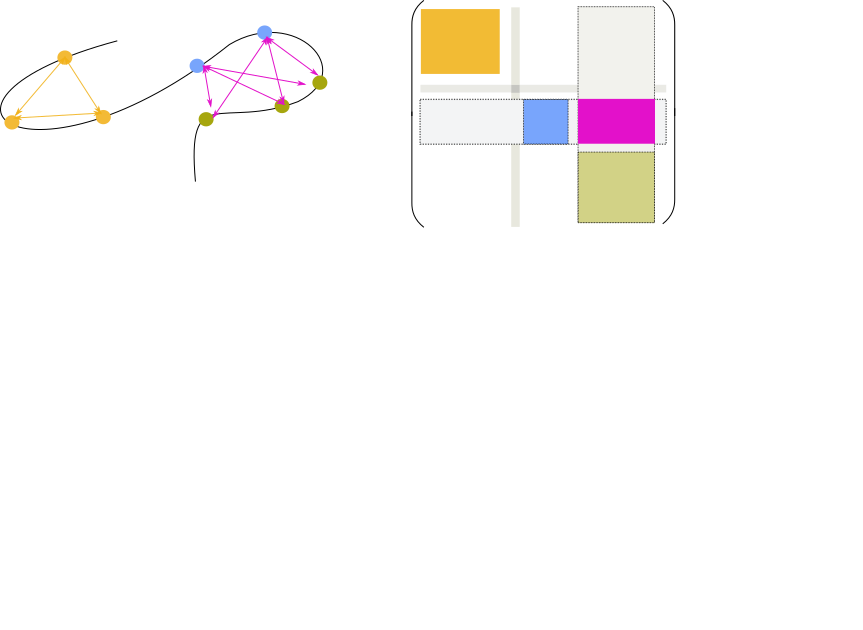
\includegraphics[width=12cm]{graphe/proteus/grp_matrix.png} &
     \end{tabular}
     
     \caption{Les principales structrures \og physiques\fg dans proteus}
\label{graph:struct_Phy}
   \end{figure}
   

   

\subsection{modèle de données} 


   \begin{figure}[t]
     \centering
     \begin{tabular}{cc}
       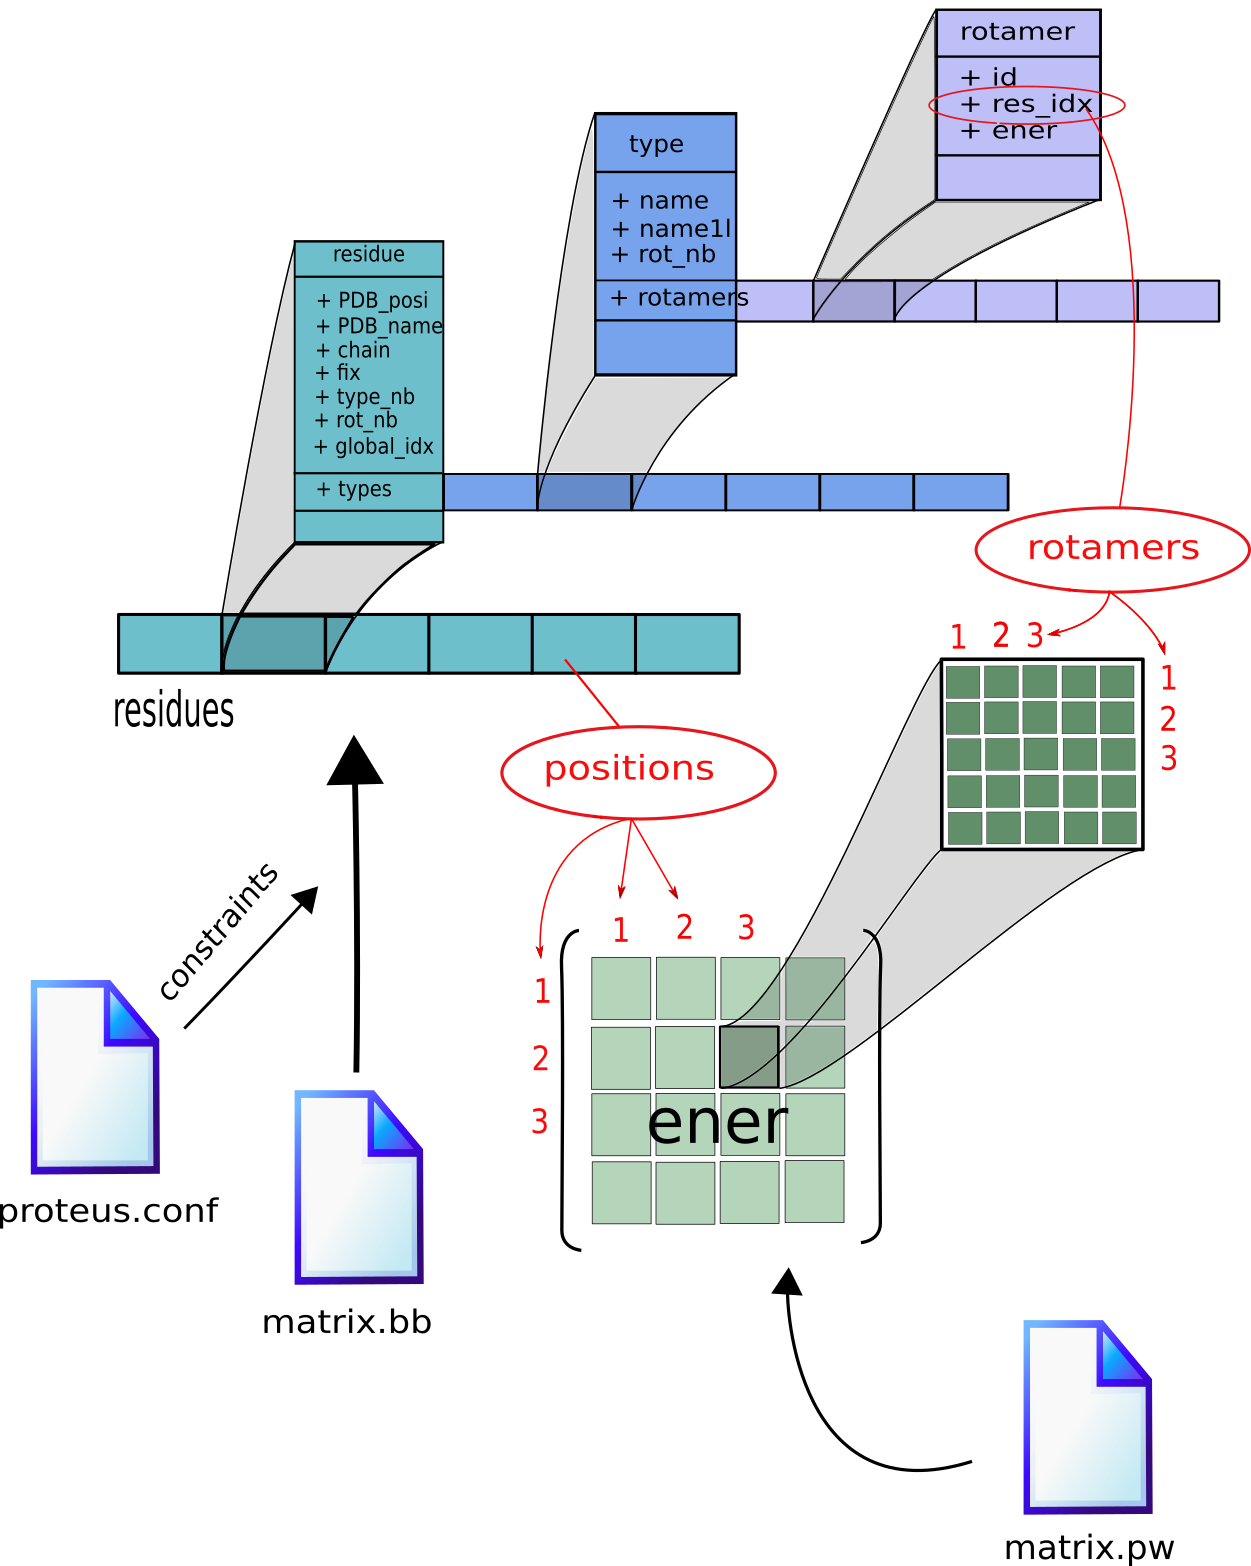
\includegraphics[width=12cm]{graphe/proteus/structures_physique.png} &
     \end{tabular}
     
     \caption{Les principales structrures \og physiques\fg dans proteus}
\label{graph:struct_Phy}
   \end{figure}



   \begin{figure}[t]
     \centering
     \begin{tabular}{cc}
       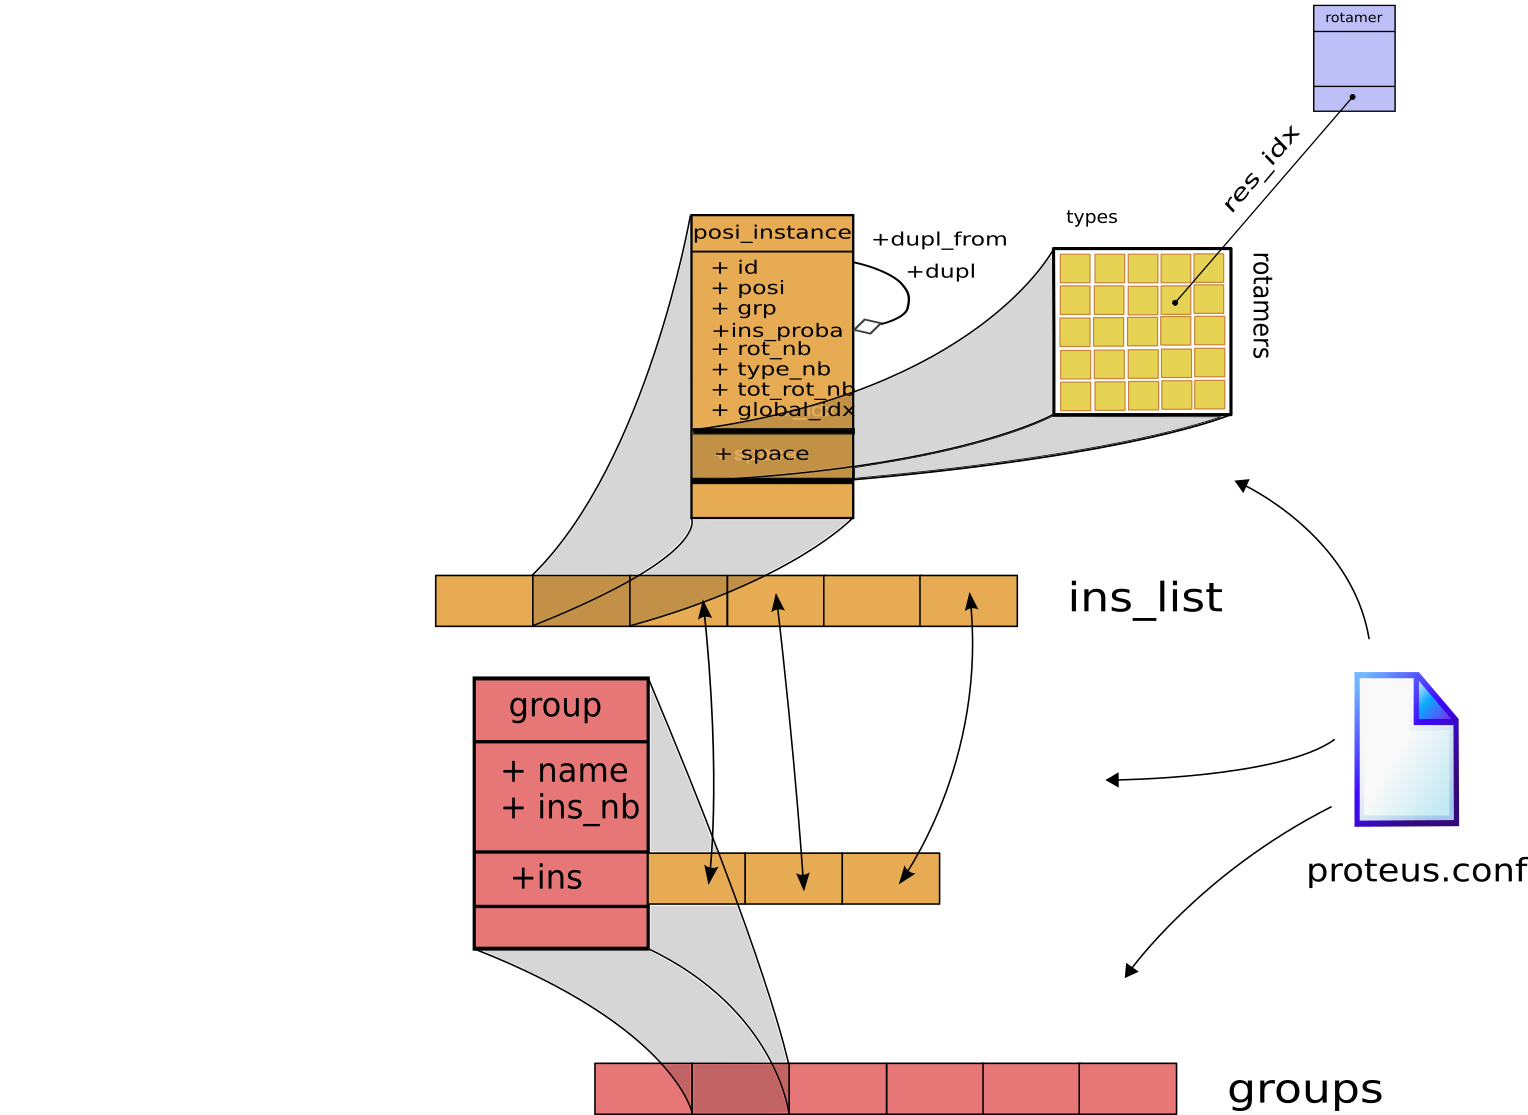
\includegraphics[width=12cm]{graphe/proteus/structures_modele_logique.png} &
     \end{tabular}
     
     \caption{Les principales structrures \og logiques\fg dans proteus}
\label{graph:struct_log}
   \end{figure}



   \begin{figure}[t]
     \centering
     \begin{tabular}{cc}
       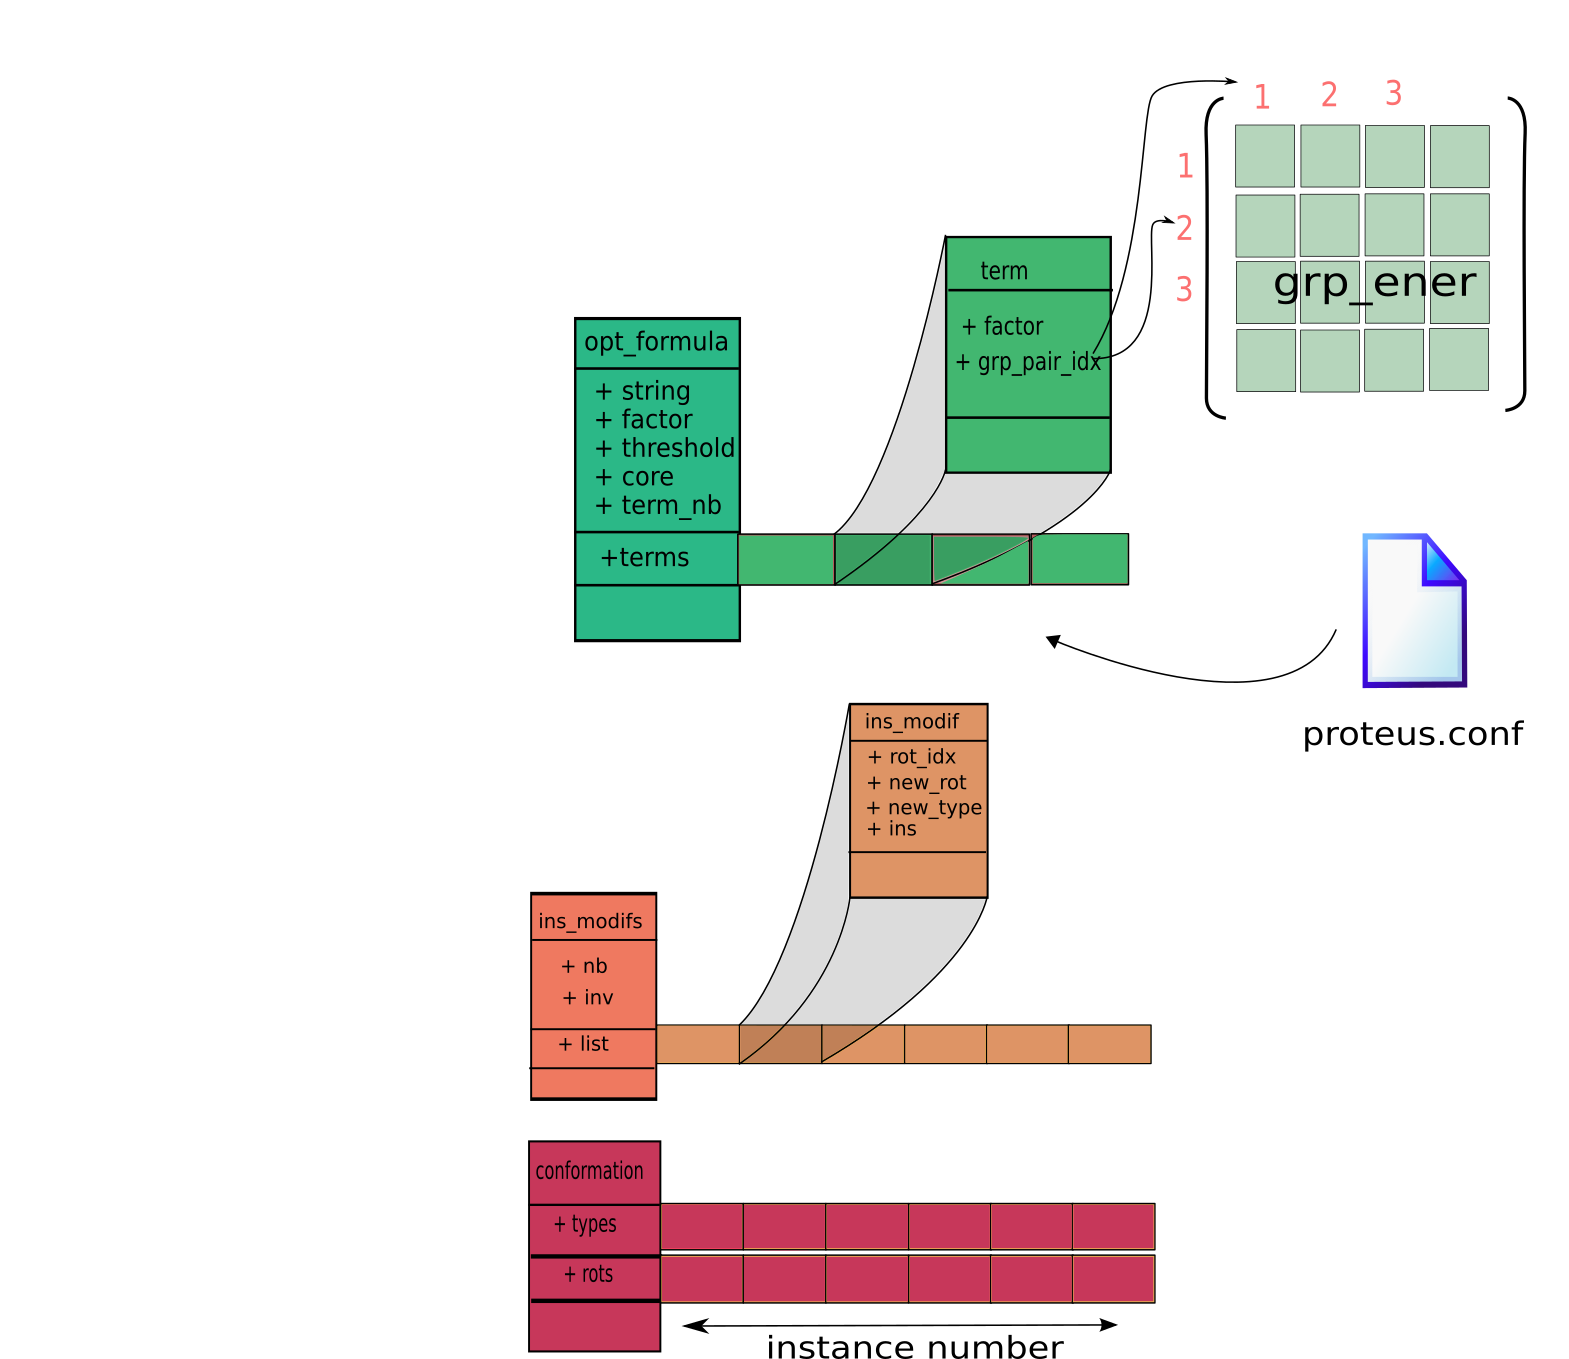
\includegraphics[width=12cm]{graphe/proteus/structures_dynamiques.png} &
     \end{tabular}
     
     \caption{Les principales structrures \og dynamiques\fg dans proteus}
\label{graph:struct_Dyna}
   \end{figure}

   

\subsection{Les entrées\_sorties} 


\paragraph{Le fichier de configuration}




    \begin{table}[!htbp]
      \centering


      \begin{tabular}{|p{0.2\linewidth}|p{0.35\linewidth}|p{0.45\linewidth}|}

        \hline
        Type   & nom & Description \\
        \hline
          methode  d'exploration & Mode &  determine  le mode d'exécution, les valeurs possibles sont HEURISTIC,MONTECARLO,MEANFIELD et POSTPROCESS  \\  \hline    
                        & Trajectory\_Length  &  la longueur de la trajectoire MC ou REMC\\  \cline{2-3}
        nombre de pas & Trajectory\_Number  &  le nombre de trajectoire  MC ou REMC  \\  \cline{2-3}
                        & Cycle\_Number  &    le nombre de cycle en mode HEURISTIC   \\ \cline{2-3}  
                        & Sequence\_Pass\_Number  &  le nombre maximum d'iteration sur  la structure à chaque cycle(mode HEURISTIC)    \\ \hline  

        fonction d'énergie &  Optimization\_Configuration &   definition de la fonction d'énergie\\               \cline{2-3}
                        &  Group\_definition &   groupes  d'energies et d'énergies d'interactions,ce sont les éléments de base de la fonction d'énergie\\  \hline  
        restrictions de l'espace de  sequence/rotamer & Space\_Constraints   &  restraint les états visités \\ \hline                
                         
     paramètre du modèle & Temperature & attribue les températures aux marcheurs MC  \\          \hline     
                         & Random\_Generator &  Le générateur de nombre aléatoire de la \og GNU Scientific Library \fg \\ \cline{2-3}
                         & Rot\_Proba &  probabilité d'avoir un changement de rotamère à chaque pas \\              
        Configuration    & Rot\_Rot\_Proba &  probabilité d'avoir un double changement de rotamère à chaque pas\\          
        Monte Carlo      & Mut\_Proba &  ... \\              
                         & Mut\_Mut\_Proba & ... \\              
                         & Mut\_Rot\_Proba & ... (ancienne version de Proteus)\\             \cline{2-3}  
                         & Position\_Weights  & probabilité de tirage de chaque position, lors de la première choix\\  
                         & Step\_Definition\_Proba  & probabilté de changer un rotamère ou un type d'aa\\   \cline{2-3}
        
                         & Neighbor\_Threshold & à chaque pas les changement se font dans le même voisinnage énergétiques.Cette balise définit la taille des voisinnages.\\   \hline
        
                         & Fasta\_File & le nom du fichier produit par le mode POSTPROCESS\\    \cline{2-3}             
        Input/Output     & Seq\_Output\_File & le nom  du fichier de séquences produit par le mode HEURISTIC ou MONTECARLO\\    \cline{2-3}             
                         & Energy\_Output\_File & le nom du fichier d'énergie produit par le mode  HEURISTIC ou MONTECARLO\\   \hline              

      \end{tabular} 

      \caption{ Une partie des balises possibles dans le fichiers de configuration de Proteus}      

      \label{table1}

  \end{table}





\paragraph{Les fichiers \og backbone\fg et \og parwise\fg}


   \begin{figure}[t]
     \centering
     \begin{tabular}{cc}
       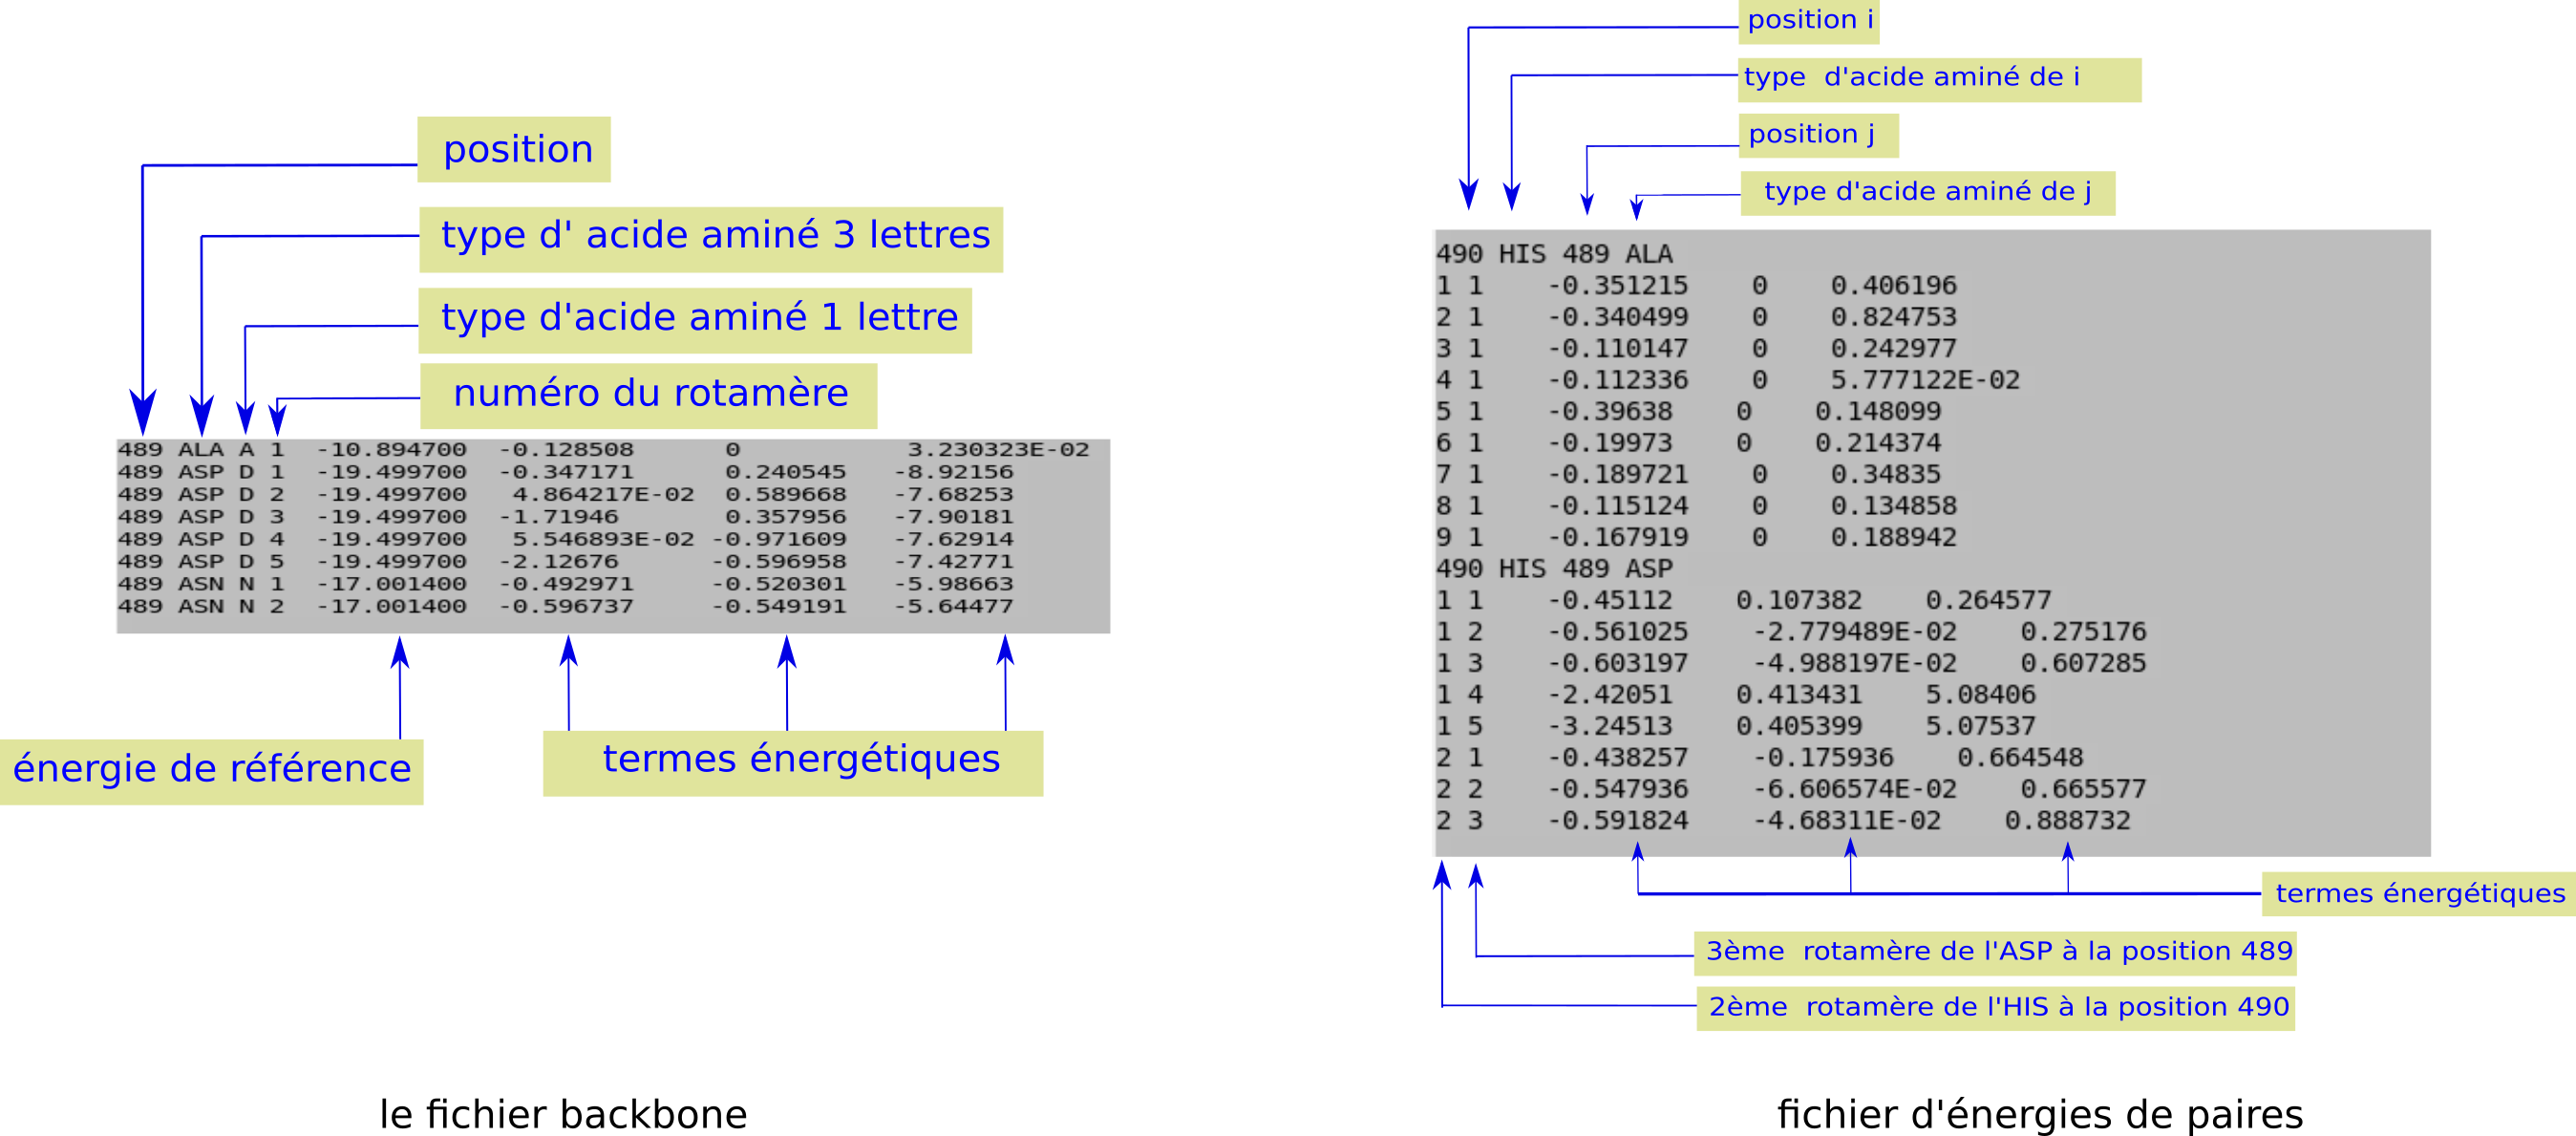
\includegraphics[width=12cm]{graphe/proteus/inputener.png} &
     \end{tabular}
     
     \caption{Les fichiers en entrée}
\label{graph:struct_Phy}
   \end{figure}



\paragraph{Les fichiers de sortie}
   
   \begin{figure}[t]
     \centering
     \begin{tabular}{cc}
       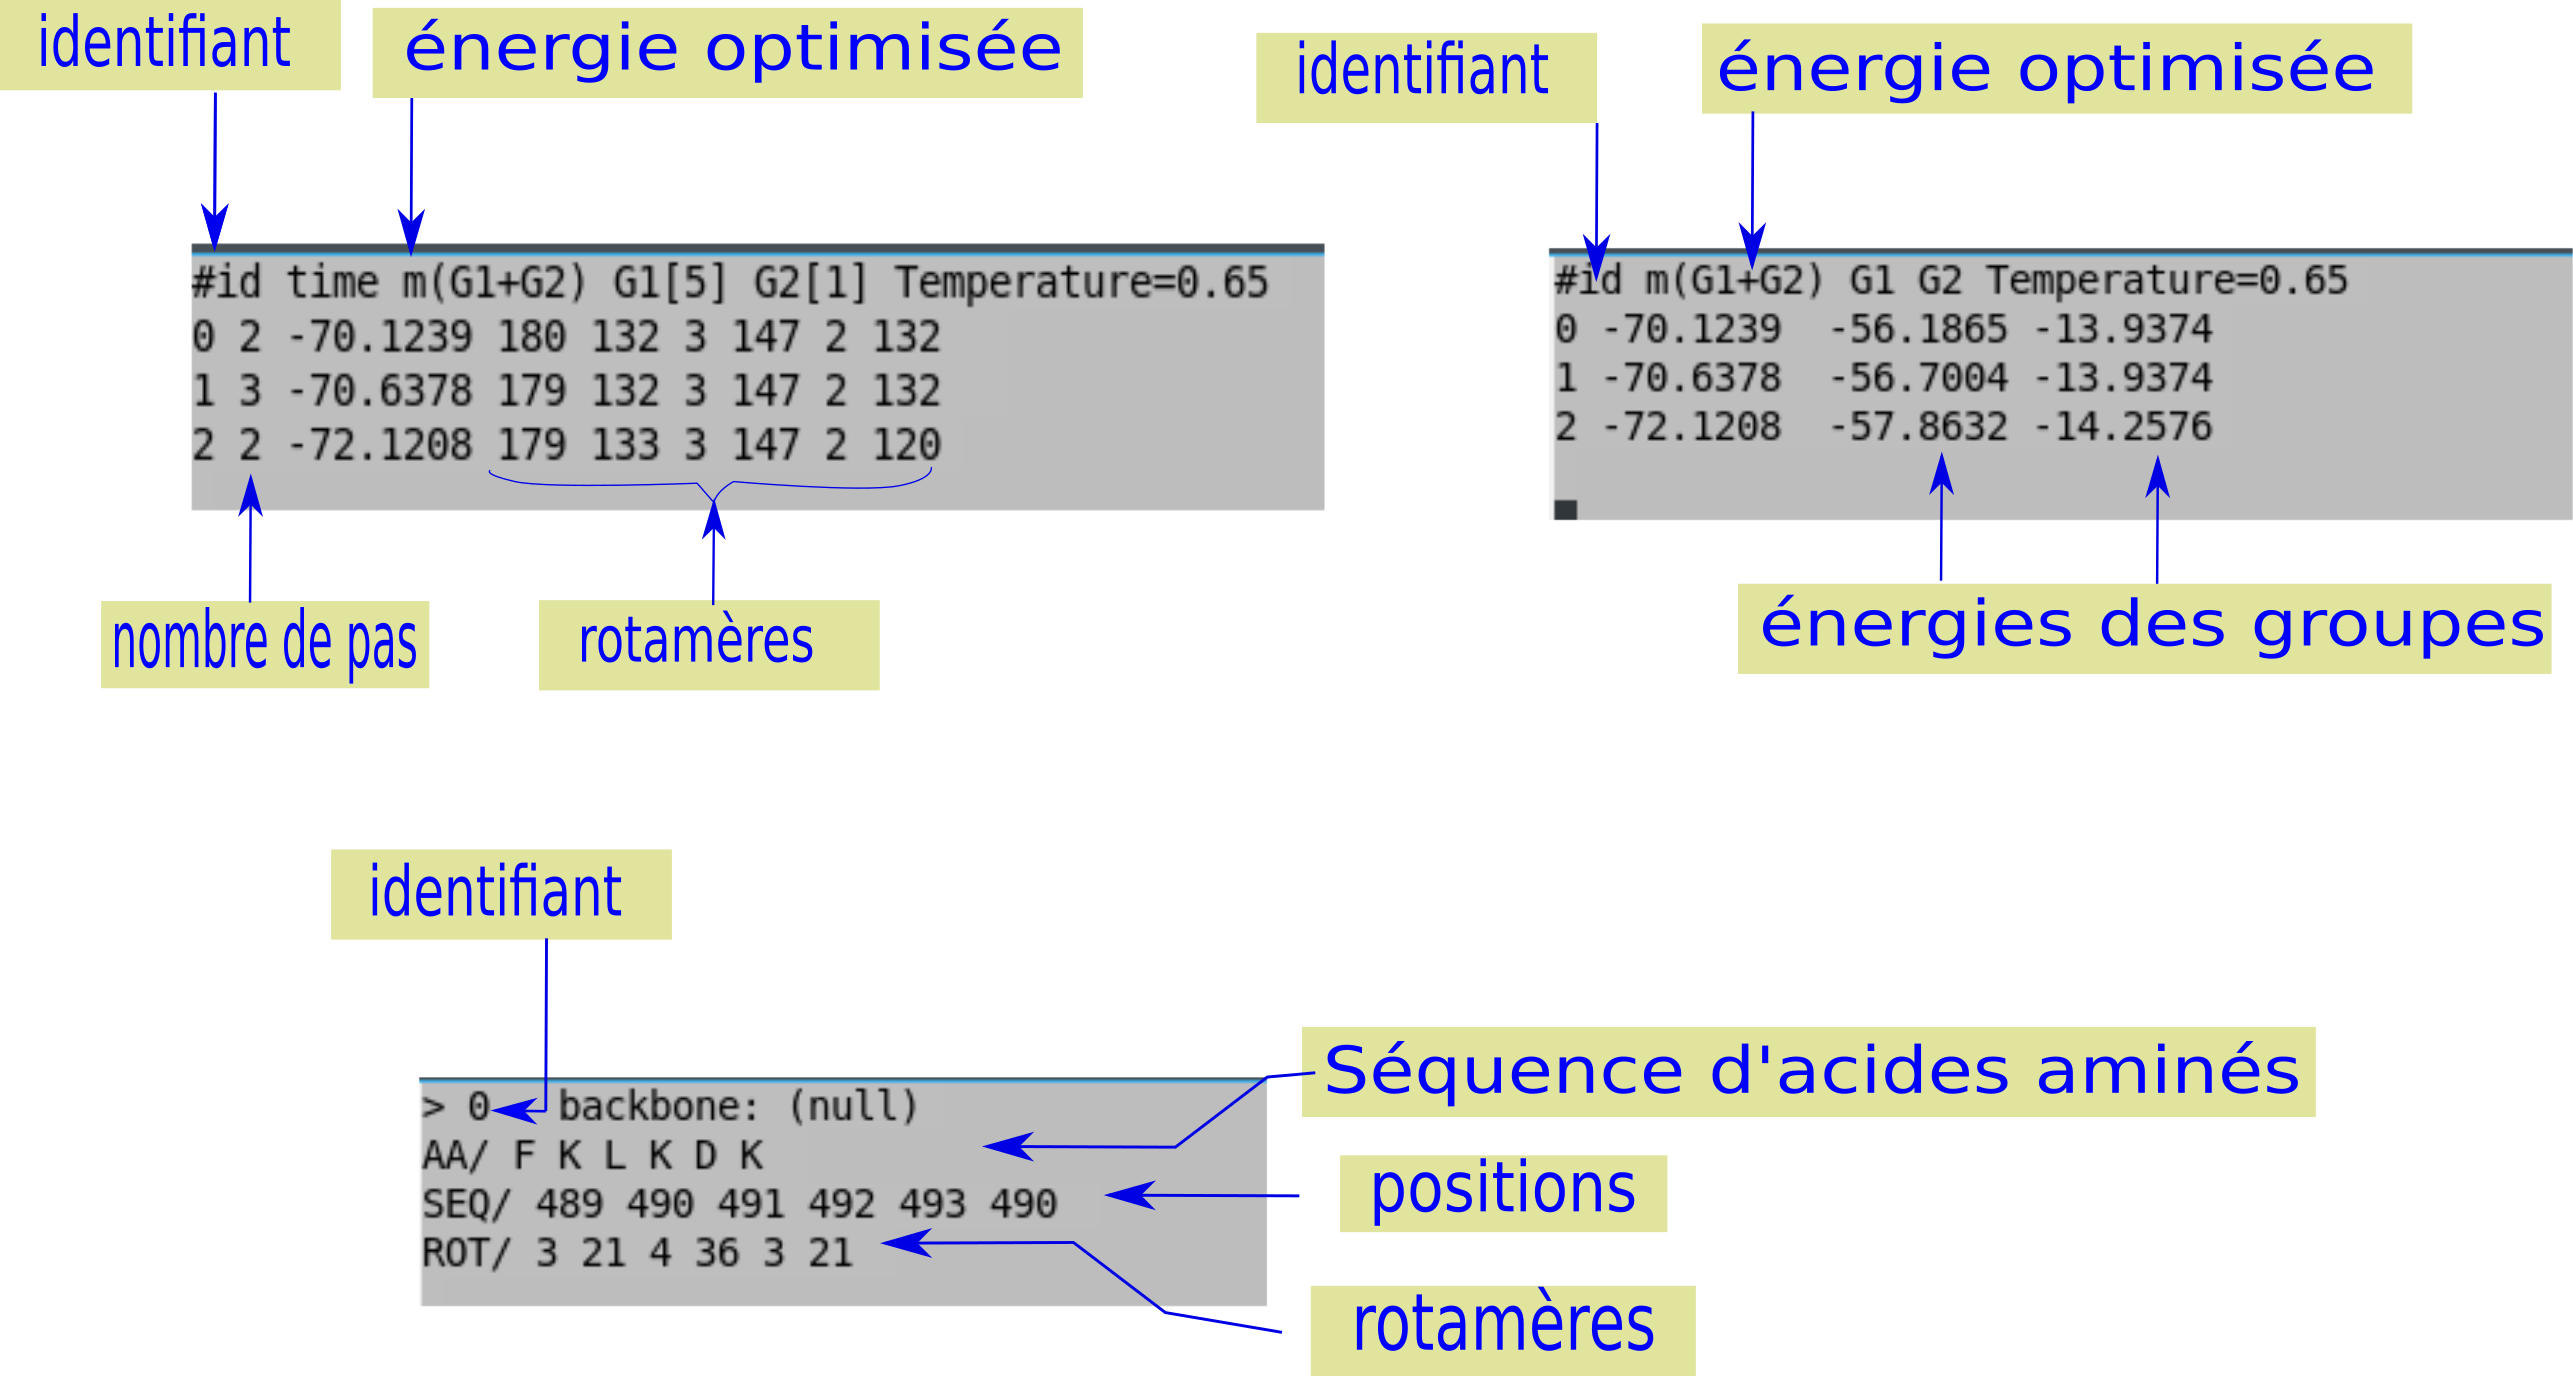
\includegraphics[width=12cm]{graphe/proteus/output.png} &
     \end{tabular}
     
     \caption{Les fichiers en sortie de proteus}
\label{graph:struct_Phy}
   \end{figure}
   

\section{Description des tests de comparaisons d'algorithme} 
\label{sec:methodes_pratiques}
Nous cherchons maintenant à déterminer les performances et les qualités des différents algorithmes de proteus.
Pour évaluer les différents algorithmes de proteus, comme pour leur établir un paramétrage, nous effectuons des séries de tests. 
Grâce à l'algorithme de type toulbar2 il est possible d'obtenir la séquence/conformation qui possède la plus haute énergie de dépliement. Cela constitue une information important qui va nous servir d'élément de comparaison.Le facteur temps est également un élément déterminant. Il est dans certain cas limitant, nous ne savons pas à l'avance quand toulbar2 termine. Et il apparaît d'emblée illusoire d'espérer voir ce programme converger dans toutes les situations intéressantes dans un temps raisonnable.D'autres métriques qui caractérisent les séquences d'acides aminés de meilleurs énergies obtenues seront également utilisées pour les évaluations et pour les paramétrages.   

Dans la suite, on appelle «position active», une position pour laquelle, tous les types d'acides et tous les rotamères de chaque type d'acide aminé sont autorisés, au court de la recherche de proteus. On désigne «séquence/conformation» une séquence d'acides aminés munie à chaque position d'un rotamère (le backbone étant de toute façon fixé).Tandis ce que le terme simple «séquence»  sans plus de précision désigne une séquence d'acides aminés.


\subsection{Sélection des positions}

Nous cherchons à déterminer les performances et les qualités des différents algorithmes d'exploration de proteus.
Pour évaluer les différents algorithmes, comme pour leur établir un paramétrage, nous effectuons des séries de tests. 
Grâce à l'algorithme de type toulbar2 il est possible d'obtenir la séquence/conformation qui possède la plus haute énergie de dépliement. Cela constitue une information important qui va nous servir d'élément de comparaison.Le facteur temps est également un élément déterminant. Il est dans certain cas limitant, nous ne savons pas à l'avance quand toulbar2 termine. Et il apparaît d'emblée illusoire d'espérer voir ce programme converger dans toutes les situations intéressantes dans un temps raisonnable.D'autres métriques qui caractérisent les séquences d'acides aminés de meilleurs énergies obtenues seront également utilisées pour les évaluations et pour les paramétrages.   

Dans la suite, on appelle «position active», une position pour laquelle, tous les types d'acides et tous les rotamères de chaque type d'acide aminé sont autorisés, au court de la recherche de proteus. On désigne «séquence/conformation» une séquence d'acides aminés munie à chaque position d'un rotamère (le backbone étant de toute façon fixé).Tandis ce que le terme simple «séquence»  sans plus de précision désigne une séquence d'acides aminés.

\label{sec:description_tests}
Les tests sont répartis en deux ensembles:
\begin{enumerate}
\item un ensemble de tests où toutes les positions de la séquence sont actives (cela correspond aux situations de design complet de protéines) 
\item un ensemble de tests où le nombre de positions actives est gardé sous contrôle de façon à maîtriser la taille de l'espace d'exploration
\end{enumerate}


\paragraph{Ensemble «Tout actif»}
\label{methode_TTactif}
Pour le premier ensemble de tests,la totalité de la matrice d'énergie est exploitée et pour chaque position l'espace d'exploration correspond à l'espace d'état déclaré dans le fichier ".bb".C'est-à-dire que tous les types de résidu et tous les rotamères sont possibles à chaque position.
Comme l'espace des séquences/conformations à explorer est gigantesque, nous ne faisons pas de tentatives de recherche du GMEC  par méthode exacte. 

Nous effectuons des recherches avec les algorithmes suivants:

\begin{itemize}
\item heuristique, noté H par la suite;
\item Monte-Carlo, noté MC;
\item «Replica Exchange», noté RE);
\end{itemize}


\paragraph{L'ensemble «nombre d'actifs limité»}

L'ensemble «Nombre d'actifs limité» est composé de six groupes de tests avec un nombre de positions actives fixe définit de la façon suivante:  


\begin{enumerate}
\item aucune position active
\item une position active 
\item cinq positions 
\item dix  positions 
\item vingt positions 
\item trente positions 
\end{enumerate}

Lorsqu'une position n'est pas active,l'acide aminé de la position est fixé en utilisant l'acide aminé de la séquence native. La chaîne latérale est, elle, laissée libre. Il n'y a donc jamais dans nos tests de position où l'état est complètement fixé.

Le groupe «aucune position active» n'est constitué que d'un test par algorithme pour chaque protéine. Il y a donc neuf tests par algorithme.
Ce sont les tests pendant lesquels la séquence d'acides aminés est fixe et correspond à la séquence native de la protéine.

Pour les tests avec une seule position active, comme des temps de calcul le permettent, nous décidons d'être exhaustifs:
Toutes les positions sont testées, il y a alors huit cent quatre tests par algorithme.
Pour tous les autres groupes de tests (cinq,dix,vingt et trente positions actives), cinq tests sont effectués par protéine, c'est-à-dire quarante-cinq tests par algorithme.

\paragraph{le choix des positions actives}
\label{para:choix_posi}
Pour définir complètement les tests, il reste maintenant à décrire le choix des positions actives pour les groupes de numéro trois jusqu'à six.
Il y a peu d'intérêt à tester des situations avec des positions actives sans interaction entre-elles.
En effet, s'il existe une position active P dont chaque résidu est sans interaction avec tous les résidus possibles des autres positions actives, déterminer le meilleur état pour P est proche du test du groupe 2 avec P comme position active. Toutefois, cela n'est pas exactement la même question, parce que les positions actives différentes de P peuvent influencer la position de la chaîne latérale de positions inactives qui à leur tour peuvent influencer l'état de P.
Ainsi, le choix des positions actives ne se fait non pas par tirage aléatoire, car le risque d'obtenir des positions avec peu d'interactions est trop grand. Il se fait sous contrainte d'interaction.

\paragraph{positions en interactions}
Pour cela, nous utilisons la notion de voisinage de proteus. Elle se définit de la façon suivante:  
Deux positions P et Q sont en interactions s'il existe un rotamère $r_P$ de P et un rotamère $r_Q$ de Q tels que:
\begin{displaymath}
 | E(r_P,r_Q) | > S_{Vois}
\end{displaymath} 
avec $S_{Vois}$ un seuil donné par l'utilisateur à la configuration de proteus (voir chap. ?? pour les détails).

Alors on appelle «n-uplet en interaction» la donnée de n positions avec $n \in \{5,10,20,30\}$ et d'un seuil  $S_{Vois}$  tels que pour toute paire de positions (P,Q) du n-uplet, P et Q sont en interactions.
\paragraph{choix des  positions actives}
Pour définir les positions actives,nous exécutons proteus en mode verbeux, sans effectuer d'optimisation.Pour cela,
il existe plusieurs façons de procéder, ici nous utilisons le mode Monte-Carlo avec une trajectoire de zéro pas. Ces exécutions produisent en sortie standard la liste des voisins pour chaque position au seuil donnée en paramètre.
Pour chacune des neuf protéines, nous exécutons proteus avec $S_{Vois}$ égal à dix, cinq et un à tour de rôle; trois listes de voisins sont obtenues. 
Ensuite,un script dédié recherche dans ces listes, les n-uplets en interaction, en partant de la liste de voisins au sens le plus fort, c'est-à-dire dix, vers celle  au sens le plus faible ($0.1$).La recherche s'arrête lorsque cinq n-uplets au moins sont trouvés.

Nous obtenons quarante-cinq n-uplets pour le groupe à cinq (respectivement dix, vingt et trente ) positions actives pour un seuil $S_{Vois}$ égal à dix (respectivement dix, un et un). Les positions actives de tous les tests sont en annexe~\ref{chap:annexe1 }).Pour chaque n-uplet, un fichier de configuration de proteus est créé dans lequel la balise <Space\_Constraints> fixe les positions inactives en utilisant le type d'acide aminé présent dans la séquence native. 


\subsection{Définition de protocole comparable}
\label{sec:proto_compa}
Nous voulons comparer les algorithmes très différents. Un algorithme peut garantir l'obtention du minimum global en énergie (GMEC) si l'exécution se termine, mais ne garantit pas qu'elle se termine. Un autre permet un contrôle très fin du temps d'exécution sans garantie du GMEC, et d'autres enfin ont des objectifs plus large que la seule obtention du GMEC.
Mais le GMEC reste le meilleur point de commun. Nous allons donc y concentrer une part importante des comparaisons.

Nous devons noter également que l'obtention du GMEC est théorique, en pratique nous n'avons pas de preuve que le code de l'algorithme exact que nous utilisons n'a pas de bogue. Cependant,nous mettons de côté cette éventualité et dans toute la suite GMEC désigne aussi bien le minimum global en énergie que le résultat de toulbar2 lorsqu'il se termine.  
Le Monte-Carlo et le «Replica exchange» possèdent de nombreux paramètres de configuration, ce qui rend l'ensemble des protocoles possibles très grand. Se pose alors la question de l'optimisation du protocole. L'objectif fixé ici,n'est pas la recherche d'un protocole optimal pour chacun des tests, mais d'évaluer, avec les tests, un protocole optimisé par algorithme.
Nous allons alors dans un premier temps, recherche les meilleurs paramétrages pour le Monte-Carlo et le «Replica Exchange» sur l'ensemble de tests «tout actif».
Puis, sur la base des résultats obtenus, les protocoles seront fixés pour effectuer les comparaisons sur l'ensemble  «tout actif» et celui à «nombre d'actifs limité».
Le programme toulbar2 possède aussi de nombreuses options. Deux paramétrages différents seront utilisés.

Pour rendre les protocoles comparables, le temps d'exécution maximum est fixé à vingt-quatre heures pour tous les exécutions.
Toulbar2 donne sa meilleure séquence/conformation en dernier, il n'y a donc pas post-traitement nécessaire.
C'est également le cas pour le Monte-Carlo à condition de configurer l'impression de la trajectoire avec la balise $Print\_Threshold=0$. dans le fichier de configuration.
Pour le "Replica Exchange" et l'heuristique, un tri des séquences selon l'énergie est nécessaire. Mais il n'y a pas beaucoup de séquences: 
\begin{enumerate}
\item L' Heuristique fournit une séquence/conformation à chaque cycle.
\item Le "Replica Exchange avec $Print\_Threshold=0$ produit autant de fichiers de séquences/rotamères que de marcheurs.Chacun ne contenant pas plus de quelques dizaines de séquences/rotamères. 
 \end{enumerate}

Nous pouvons donc négliger la durée du tri dans le temps total d'exécution.    

\paragraph{Protocole heuristique}

Pour l'algorithme heuristique, il n'y a dans notre situation qu'un seul paramètre à renseigner: le nombre de cycles à effectuer. Quelques essais préliminaires sur la plus grosse protéine (Table~\ref{tab:protéines}) avec toute les positions actives, montre que la version utilisée de proteus peut effectuer jusqu'à environ 110000 cycles sur nos machines de calculs en l'espace de vingt-quatre heures. Ainsi, le protocole H est défini comme le protocole qui utilise le mode heuristique de proteus et qui effectue cent dix mille cycles. Sont également définis les variantes H-, H+ et H++ comme des protocoles plus courts ou plus longs à facteur entier près (Table~\ref{tab:protoH}). Par ailleurs, certaines comparaisons de l'heuristique avec le Monte-Carlo ont été faites avec une version précédente du programme proteus.Ce protocole sera noté h. Il diffère aussi de H par le fait que l'option d'optimisation du compilateur Intel utilisé est -O2 contre -O3 pour H.    


   \paragraph{Protocoles Monte-Carlo}
\label{para:MC}
On distingue deux ensembles de protocoles Monte-Carlo.Dans le premier, les noms  sont de la forme "mc*". Il rassemble les protocoles utilisés pour le paramétrage du Monte-Carlo.Le second est constitué des protocoles utilisés lors des comparaisons.     

Les éléments à paramétrer pour l'algorithme Monte-Carlo sont les suivants:

\begin{enumerate}
\item la température
\item le nombre de pas (avec le nombre de trajectoires et la longueur de trajectoire )
\item Le seuil de voisinage
\item Les probabilités de changements de la séquence/conformation
\end{enumerate}

Ce qui représente un ensemble de protocoles trop grand pour une approche exhaustive. Pour l'essentiel, nous allons faire varier les paramètres un par un, en prenant comme point de départ un protocole qui rend le comportement de marcheur Monte-Carlo «proche» de l'heuristique.

La température est le paramètre principal du Monte-Carlo, c'est elle qui contrôle le taux d'acceptation du critère de Metropolis.Alors,la première étape de cette optimisation va consister à faire varier la température , entre 0.001 et 0.5 , en conservant les autres paramètres fixés (protocoles de mc0 à mc5).Le nombre de pas total effectué est le produit de deux paramètres, le nombre de trajectoires et la longueur de trajectoire. Les protocoles mc1b et mc2b testent l'effet d'une augmentation du nombre de pas. Tandis que mc2c et mc2d testent l'effet de la variation du nombre de trajectoires par rapport à la longueur.
Le protocole mc2e s'intéresse aux probabilités de changement de la trajectoire. Il y a cinq balises dans proteus qui contrôle ces changements:

\begin{description}
\item[<Prot>] donne la probabilité de modifications de  rotamère à une position.
\item[<Prot\_Prot>] donne la probabilité de modifications de  rotamère à deux positions.
\item[<Mut>] donne la probabilité de modifications de type de résidu à une position.
\item[<Mut\_Prot>] donne la probabilité de modifications de  rotamères à deux positions.
\item[<Mut\_Mut>] donne la probabilité de modifications de type de résidu à deux positions.
\end{description}

La table~\ref{tab:protoMC} donne les probabilités utilisées par ces cinq paramètres dans l'ordre de la liste précédente. 

Enfin, mc4b se distingue des autres par un seuil de voisinage plus grand ((Table~\ref{tab:protoMC})).

   \paragraph{Protocoles "Replica Exchange"} 

L'algorithme «Replica Exchange» (RE) est une extension du Monte-Carlo. Les paramètres d'un protocole RE sont ceux d'un protocole Monte-Carlo plus trois autres:

\begin{itemize}
\item le nombre de marcheurs
\item la température pour chaque marcheur
\item la période de «swap», c'est-à-dire la période (en nombre de pas) à laquelle le test de Hasting sur l'échange de température est effectué.
\end{itemize}
Pour avoir des exécutions en parallèle avec au plus un marcheur par coeur du processeur, nous limiter nos tests à quatre ou huit marcheurs.
La distribution des températures est un élément déterminant dans le comportement des marcheurs, car c'est elle qui pilote en grande partie le taux d'acceptation des échanges de températures. Nous suivons l'idée proposée par Kofke de lui faire suivre une progression géométrique ( $ \frac{T_i}{T_{i+1}}=C $ , avec C une constante)~\citep{refRE1,refRE2,refRE3}. Ceci garantie alors que le taux d'acceptation d'échange entre $T_i et T_{i+1}$ soit égale pour tout nos i.De plus, nous souhaitons centrer approximativement, nos distributions sur la température ambiante (environ 0.6 kcal/mol). Dans toute la suite, les températures et les énergies sont exprimées en kcal/mol.

Voici les températures pour le RE quatre marcheurs:

\begin{itemize} 
\item 10, 1, 0.1 et 0.01
\item 2, 1, 0.5 et 0.25 
\item 1, 0.5, 0.25 et 0.125
\end{itemize} 

,et celles pour le RE huit marcheurs:

\begin{itemize} 
\item 3 , 2 , 1.333 , 0.888 , 0.592 , 0.395 , 0.263 et 0.175 
\item 10 , 3.16 , 1 , 0.316 , 0.1 , 0.0316 , 0.01 et 0.00316
\end{itemize} 

Ici les protocoles ne se font qu'avec une seule trajectoire par marcheur. Et la contrainte du temps de calcul se comprend comme vingt-quatre heures de calculs cumulées sur tous les marcheurs.
Ainsi les longueurs de trajectoire sont définit pour le RE à quatre marcheurs comme le quart d'une trajectoire MC, pour le RE à huit marcheurs comme le huitième.


\paragraph{Distribution des énergies en fonction des températures}

Regardons plus en détail le comportement du programme pour l'algorithme "Replica Exchange". Notre implémentation de cet algorithme consiste à modifier la température de certains marcheurs à certains moments voir~\ref{???}.Pour examiner la trajectoire à une température donnée t ( c'est à dire le graphe dans l'espace les séquences/conformations selon les pas du marcheur lorsqu'ils sont à la température t), nous découpons les trajectoires des marcheurs  selon la température. Puis nous collons les segments de trajectoires de même température en respectant l'ordre des pas.Comme les changements de températures se font de façon synchrone , c’est-à-dire un échange entre deux marcheurs, nous obtenons autant de trajectoires selon la température qu'il y a de marcheurs et ces nouvelles trajectoires sont de mêmes longueurs que les trajectoires obtenues par proteus. La figure~\ref{graph:Distrib_E_T} représente la distribution en énergie des trajectoires selon la température sur le test utilisant le protocole RE8b1 sur la protéine 1A81. Nous observons une courbe en cloche pour chaque température, retrouvant ainsi l'allure d'une distribution de Boltzman.  L'espace de recouvrement entre deux courbes consécutives, représente la partie de la distribution dans laquelle les échanges de température vont être se concentrer, parce que cette zone recouvre les situations où la température peut augmente sans dégradation de l'énergie. En effet, le critère de Metropolis-Hasting peut accepter un réchauffement de marcheur (respectivement un refroidissement) si son énergie diminue  (respectivement, augmente) , mais uniquement avec une probabilité qui décroît exponentiellement en fonction de la différence d'énergie.À l'inverse si les recouvrements des distributions consécutives sont trop importants le marcheur peut difficilement s'éloigner de la plage d'énergie d'une température.Le graphique nous confirme que le choix d'une plage de température entre 3.0 et 0.175 pour les protocoles huit marcheurs rend possibles les échanges de températures et permet également l'exploration d'une vaste zone d'énergie.   




   \begin{figure}[t]
     \centering
     \begin{tabular}{cc}
       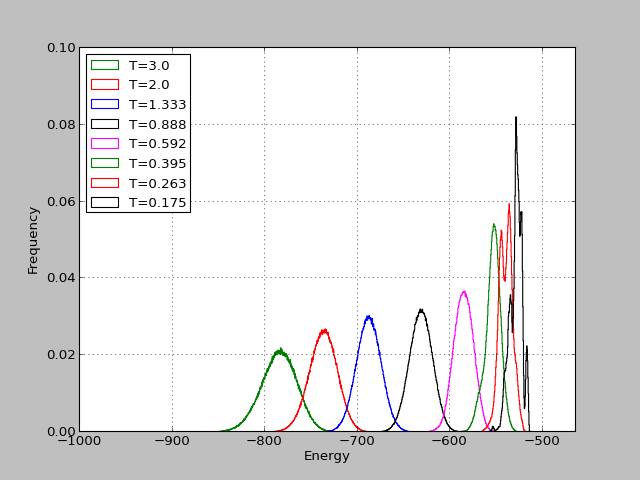
\includegraphics[width=12cm]{graphe/1A81_RE8b1.png} &
     \end{tabular}
     
     \caption{Distribution des énergies selon la température (1A81 protocole RE8b1).}
\label{graph:Distrib_E_T}
   \end{figure}

\paragraph{Trajectoires dans l'espace des températures}

Un critère de performance souvent utilisé est la proportion de changements de températures effectivement acceptés. Pour examiner ces changements, nous représentons la trajectoire dans l'espace des températures pour quatre tests sur la protéine 1A81. Il s'agit des tests effectués avec deux protocoles à quatre marcheurs, le RE4a et le RE4b et deux protocoles à huit marcheurs, le RE8a2 et le REb1, voir figure~\ref{graph:TRAJ_T}.Les deux graphiques quatre marcheurs représentent seulement la moitié des trajectoires de 1,5 million de pas , tandis que les graphiques huit marcheurs représentent la totalité de trajectoires de 750 millions de pas.Comme prévu, le protocole RE4a , qui possède des températures plus écartées , brasse assez mal les températures. En particulier, le marcheur w4 ne quitte presque pas la température la plus froide, et ce malgré une période de swap assez faible et un nombre d'échanges effectifs assez important. On voit que pour RE4b, protocole avec les températures plus proches , la répartition des échanges est nettement plus uniforme. Le fait de double le nombre de températures pour le même intervalle que RE4a ne suffit pas à résoudre le problème et les trois marcheurs les plus froids en début de trajectoire pour le RE8a2 restent froids. Les bons résultats obtenus pour RE4b sont confirmés pour RE8b1 qui utilise également des températures proches.     


   \begin{figure}[t]
     \centering
     \begin{tabular}{cc}
       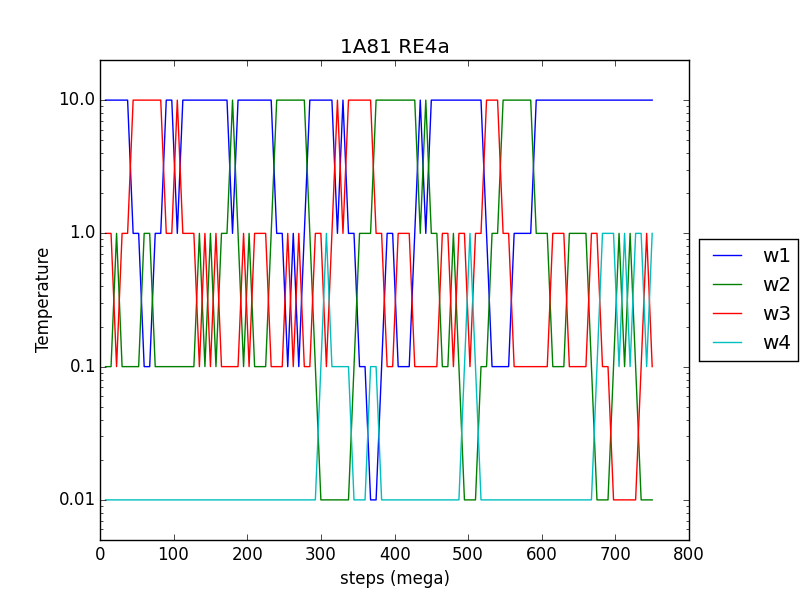
\includegraphics[width=8.45cm]{graphe/1A81-RE4a-T_traj.png} &
       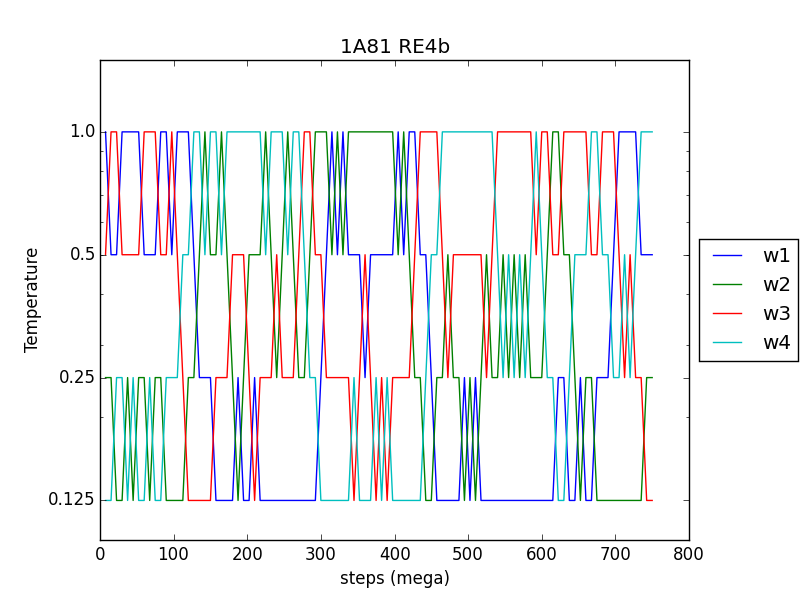
\includegraphics[width=8.45cm]{graphe/1A81-RE4b-T_traj.png} \\
       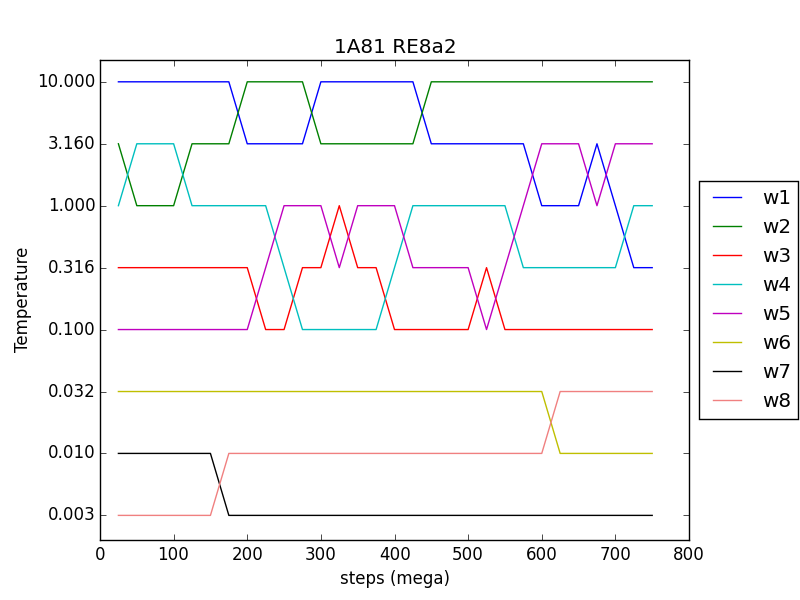
\includegraphics[width=8.45cm]{graphe/1A81-RE8a2-T_traj.png} &
       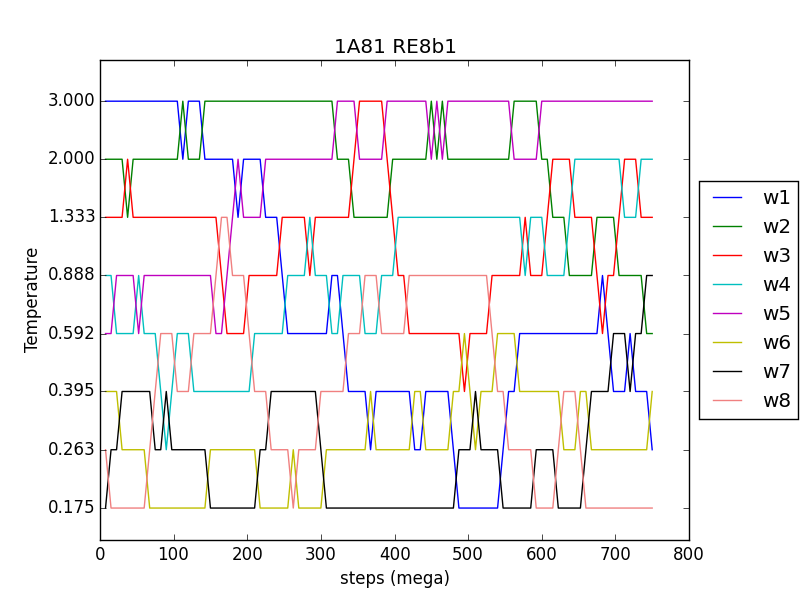
\includegraphics[width=8.45cm]{graphe/1A81-RE8b1-T_traj.png} \\
     \end{tabular}
     \caption{Variation de la température pendant la trajectoire de chaque marcheur (cas exemple de protocoles).}
\label{graph:TRAJ_T}
   \end{figure}


   \paragraph{Protocoles Toulbar2} 
\label{proto_toulbar2}

Après avoir converti nos matrices au format «wcsp» grâce à un script dédié,nous pouvons utiliser toulbar2.
Le protocole de recherche du GMEC est le suivant:
L'exécutable toulbar2 de version 0.9.7.0 est lancé avec les options « -l=3 -m -d: -s», ce qui correspond au paramétrage conseillé dans la documentation CDP~\citep{reftoulbar1,reftoulbar2}. Si l'exécution se termine en moins de vingt-quatre heures, le protocole est achevé. Sinon le programme est arrêté et une seconde version (la 0.9.6.0) est lancée avec les options «-l=1 -dee=1 -m -d: -s». Au bout de vingt-quatre heures si le programme n'est pas terminé, il est arrêté. La dernière séquence/conformation imprimée en sortie est collectée. Le choix de la seconde version et du paramétrage fait suite à une discussion avec monsieur Seydou Traoré.  

Toulbar2 offre également la possibilité de fournir la liste des séquences/conformations dont l'énergie est comprise entre celle qui correspond au GMEC, $E_{GMEC}$ et une autre $E_{upper\_bound}$ donnée en paramètre. Pour utiliser cette fonctionnalité nous utilisons le paramétrage:  «-d: -a -s -ub=$E_{upper\_bound}$ ».Cependant, il s'avère que cette utilisation peut utiliser une quantité de mémoire vive importante.Alors, pour eviter tout plantage de nos machines, la mémoire que toulbar2 peut allouer est limité à 30 Go.

\subsection{Outils d'analyse des données} 
   \paragraph{Superfamily/SCOP} 

Superfamily~\citep{refSuperfamily} est un ensemble composé: 

\begin{itemize}
\item D'une base de données de modèles de Markov cachés, où chaque modèle représente une structure 3D d'un domaine de la classification SCOP.
\item D'une série de scripts qui annotent à partir des informations de la base,les séquences données en entrée. Ici, nous utilisons uniquement l'association au modèle 3D le plus vraisemblable. 
\end{itemize}

Nous travaillons avec la base de données à la version 1.75, et en conjonction, nous utilisons SAM (version 3.5)~\citep{refSam} et HMMER (version 3.0)~\citep{refHmmer} recommandés par l'équipe de Superfamily. Le paramétrage utilisé est celui par défaut.

\paragraph{Taux d'identité de séquences}

Soient S et N deux séquences d'acides aminés de même longueur l.

Le Taux d'identité $Id(S,N)$ de S par rapport N est égal au pourcentage de position où l'acide aminé est identique dans S et N. C'est-à-dire

  $ Id(S,N) =\frac{\sum_{1<i<l} \mathds{1}(s_i,n_i)}{l} \times 100$ 

avec $s_i$ et $n_i$ l'acide animé en i de S et de N respectivement, et $\mathds{1}(x,y)$ la fonction qui vaut 1 lorsque x=y et 0 sinon. 

\paragraph{Taux d'identité par position}

Le taux d'identité d'un alignement $A_S$ à la position i par rapport à une séquence N de même longueur se définit comme:

$Id(A_{S},i) = \frac{\sum_{1<j<m} \mathds{1}(s_i^j,n_i)}{m} \times 100$ , avec m le nombre de séquences de $A_S$.

\paragraph{Alignements Pfam} 
Ce taux d'identité donne une mesure de la ressemblance entre un alignement et une séquence. Cela nous permet de comparer nos séquences calculées à la séquence native. Mais cela n'est pas notre seule objectif.Et nous voulons les évaluer par rapport à l'ensemble des séquences du domaine protéique de la native.  
La base de données Pfam (Protein families database)~\citep{refPfam} regroupe les domaines protéiques connus en famille. Chaque famille étant représentée par des alignements multiples de séquences et des profiles de modèles de Markov cachés~\citep{refPfam}. Dans la suite, nous n'utiliserons l'alignement dit « seed» qui se base sur un petit ensemble de membres représentatifs de la famille et l'alignement « full» , plus large, qui est généré par modèle de Markov caché à partir de l'alignement «seed». Les alignements correspondent pour nous aux familles PF00017 (domaine SH2), PF00018  (domaine SH3) et PF00595 (domaine PDZ).

\paragraph{Score BLOSUM}

Pour tenir compte des ressemblances et des différences entre les acides aminés lors d'une substitution, nous avons besoin d'une matrice de coût.Nous utilisons la matrice BLOSUM62 (BLOcks SUbstitution Matrix)~\citep{refBLOSUM} qui est construite à partir de blocs d'alignement très conservés (ici plus de 62\% d'identités).Les fréquences des mutations y sont calculées.Le score BLOSUM d'une substitution est alors le logarithme de la fréquence de la mutation correspondante.À cela est ajouté un score de pénalités pour l'insertion d'un gap (c'est-à-dire un saut dans l'alignement).

On définit alors simplement un score de similarité de deux séquences de même longueur comme la somme des scores BLOSUM62 sur toutes les positions. De même le score de similarité d'un alignement par rapport à une séquence sera défini comme la moyenne des scores de similarité sur ensemble des séquences de l'alignement. Et enfin un score de similarité de deux ensembles de séquences alignés entre eux comme la moyenne des scores de similarité du premier ensemble par rapport aux séquences du second.  

\paragraph{similarité d'un ensemble à une famille Pfam}

Afin de calculer un score de similarité d'un ensemble de nos séquences par rapport à une famille Pfam, il faut commencer par aligner nos séquences avec l'alignement de la famille.Pour cela nous utilisons le programme d'alignement BLAST~\citep{refBLAST}.Il implémente une heuristique qui recherche puis étend les meilleurs alignements locaux. Nous procédons comme suit:
\begin{enumerate}
\item La commande blastpgp est utilisée avec comme database (paramètre -d ) l'alignement Pfam et comme séquence en entrée ( paramètre -i ) la séquence native. 
\item Dans la sortie blast, la séquence qui produit l'alignement le plus significatif avec la native est collectée, notons-la $S_0$. 
\item L'alignement blast est alors utilisé pour positionner la native par rapport à $S_0$ et les gaps nécessaires pour aligner la native à $S_0$ sont ajoutés.
\item Le positionnement et les gaps sont alors appliqués tels quels à la liste de nos séquences.

\end{enumerate}


\clearpage


%%% Local Variables:
%%% mode: latex
%%% TeX-master: "../these"
%%% End:
